% !TEX root = rapport.tex

\section{Methods of Tomorrow}
\label{future}
Admittedly there is no way of knowing with certainty what the future has in store, and this is just as true when it comes to technical development. On the other hand, knowing what the prominent factors are, one can more easily predict this development. It can be seen that the history of input and output devices has actually not had a tight connection to that of computer processing power and memory, although the lack of which can delay the popularisation of such devices. Some examples of this are mentioned above: the computer terminal gained in popularity first when computer memory became more easily available, and the use of neural networks gained in popularity in the 1980's when processing power had increased. According to the well-known Moore's law, the number of transistors and hence chip performance doubles approximately every two years, further leading us to believe that this is not the main issue.

Development rather aspires to ease the interaction either by making devices more portable and available or to remove the obstacles present in the interaction. This is well exemplified by the \emph{Google Glass} project currently under development. The glasses are worn like traditional glasses, but have a built-in display where the glass traditionally would be, and is controlled by speech commands. This way, the system aims to provide both higher portability and more natural interaction with the user.

Taking this trend of portability and user-centered interaction into account, this section will cover two possible interaction methods likely to grow in popularity in the future: the use of gesture based systems, and systems to control devices directly by thought. 


\subsection{Gesture control}
Gesture control is a means of interaction that uses either hand-gestures or full-body gestures to control and interact with a device. In a way, this form of control aims to immitate human-human interaction by removing the need of physical interaction with a device. Possibly the first such system was the \emph{theremin} developed 1919/1920 by Leon Theremin, see figure \ref{theremin}. The theremin is an electronic musical instrument, operated by hand gestures. Depending on the position of the hands in relation to the antennas, sounds of different frequencies can be generated~\cite{thereminpatent}.

\begin{figure}[]
\center
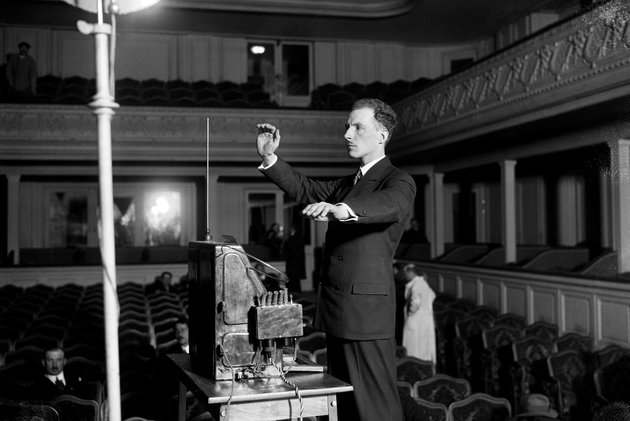
\includegraphics[width=0.8\textwidth] {bilder/teremin.jpg}
\caption{Leon Theremin operating a theremin in 1927~\cite{theremin}.}
\label{theremin}
\end{figure}

This is an early example of how hand gesture control can be useful and intuitive in \emph{certain} contexts. There are several areas where gesture control can be useful. Separating the user from the machine can be useful to protect the physical machine from abuse, as the system is worked from a distance. During a presentation, a speaker can avoid the obstructing act of changing slides manually, instead using hand gestures to signal this command. If the session is filmed, hand gestures could easily notify the camera to focus on a certain area on a blackboard, screen or object being exhibited.

Hand gestures are often useful in the same settings where voice recognition would be useful, but does not suffer from the disadvantage of being sensitive to noise and does not break the user's flow when communicating~\cite{Hardenberg01bare-handhuman-computer}. Tracking mouth movements can also aid in speech recognition, allowing speech and gesture to be used in combination~\cite{conf/icmcs/LiuK10, conf/icmcs/SarginAKOYWEYT06}.

Several difficulties involved with gesture recognition are currently under study. To be able to recognise gestures, the systems depend on a camera which needs be positioned where it can catch the relevant movements of the subject. It must also have a rather high resolution and frame frequency in order to cope with the speed of human movement. Furthermore, this must be combined with fast and accurate algorithms to detect and track movements reliably. Besides the technical issues, there is the issue of ease-of-use. A technique that aims to provide a natural interface such as that of regular human interaction must be quite tolerant -- the input must be done on the terms of the user. 

An example of a gesture based system is the \emph{SixthSense} developed at the MIT Media Lab, a mobile system which utilises a mini-projector. The camera and the projector hang around the neck of the user similar to a pendant. The camera recognises the user's hand-gestures to perform the requests, and can optionally use the projector to project data onto a surface. What is especially interesting with the SixthSense is its user interface. In a traditional system, the user interacts with a user-interface against the computer whereas the goal of the system is to use the user's normal setting -- the physical world~\cite{Mistry:2009:SWG:1667146.1667160}. Ideally, the user would interact with objects as in a natural way with the computer aiding when appropriate. An example of such an application can be seen in figure \ref{sixthsense}.


\begin{figure}[]
\center
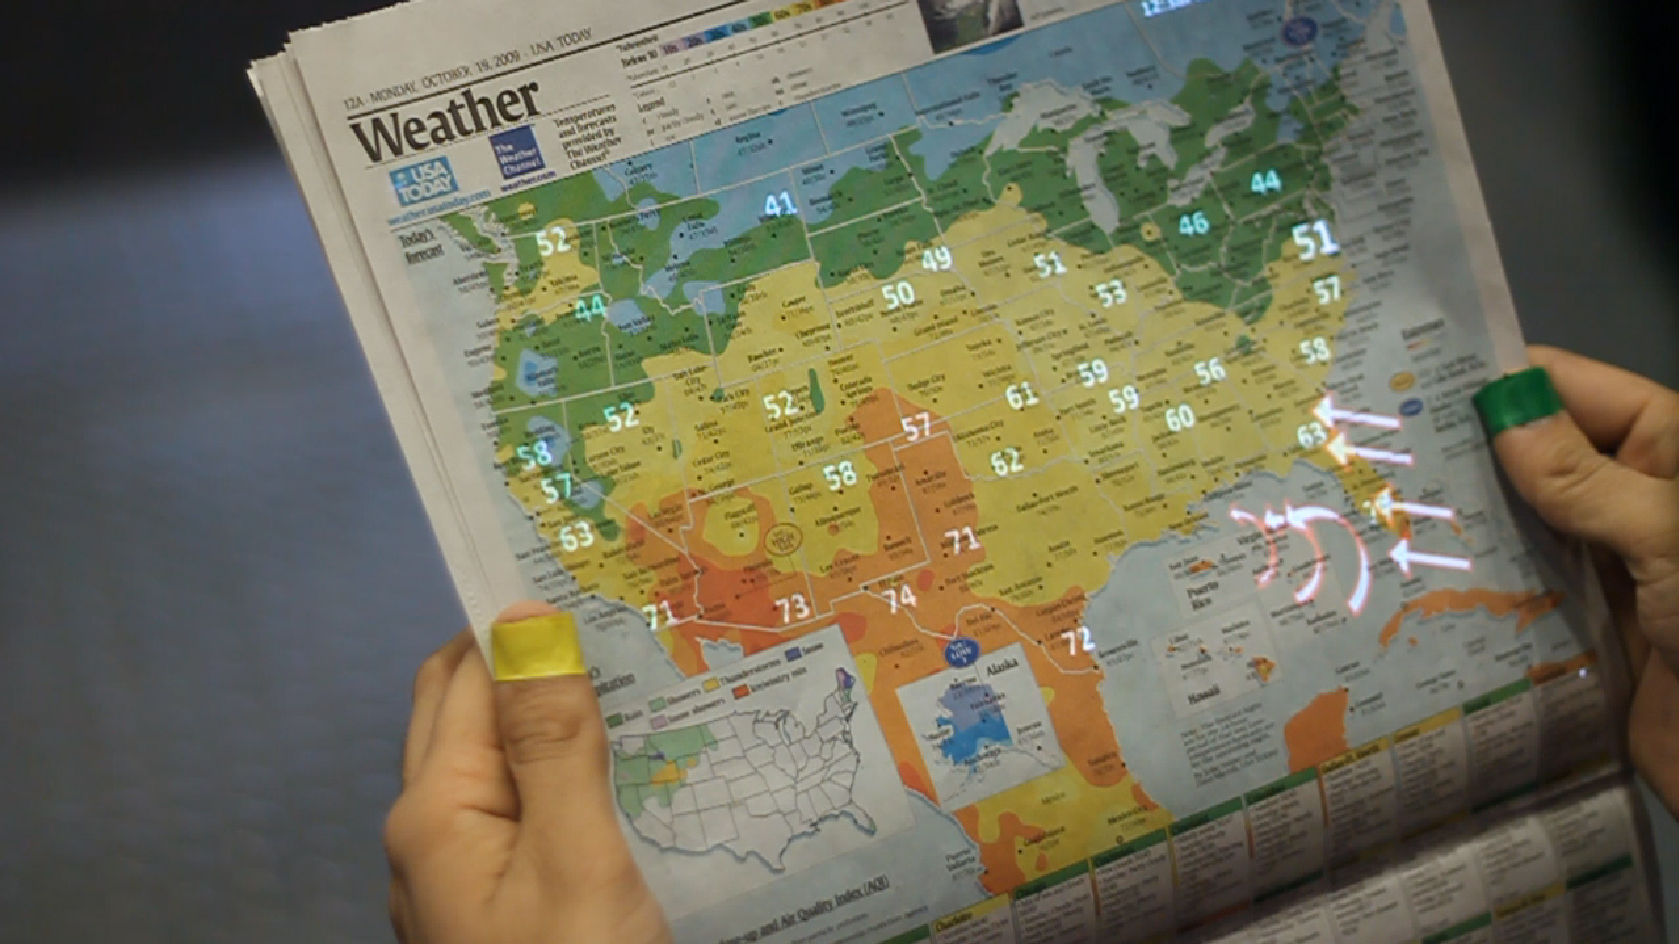
\includegraphics[width=0.8\textwidth] {bilder/newspaper.jpg}
\caption{The SixthSense interacting with a newspaper augmented with weather data~\cite{newspaper}.}
\label{sixthsense}
\end{figure}


\subsection{Brain-Computer Interfaces}

Since the early 1990's there has been a lot of research on Brain-Computer Interaction (BCI) systems~\cite{lebedev2006brain}. These systems uses brain reading techniques to use brain activity as input to a computer.

Brain-computer interaction methods can be divided into \emph{non-intrusive}, \emph{partially intrusive} and \emph{intrusive} technologies~\cite{legobrain}. Non-intrusive technologies are technologies where the brain activity reading equipment is placed on the outside of the persons head. This requires no surgical procedure and is therefore the easiest and safest method for scanning brain activity. The drawback is that the readings are usually more imprecise than intrusive methods, since the readings are distorted by the skull. However some methods~\cite{doud2011continuous} have been developed that give readings comparable to those of intrusive approaches.

The partially intrusive methods require electrodes to be placed inside the persons skull, but outside the grey matter of the brain. This approach removes the distortions caused by the skull, but require surgical procedures that can be dangerous for the patient. Intrusive methods require electrodes to be placed into the grey matter of the subject's brain. This gives the highest accuracy, down to neuron level, but can cause tissue scarring on the person, since the body tries to get rid of the foreign object.

The history of brain activity reading started in 1924 when Hans Berger discovered the electrical activity of the brain and the first EEG equipment was constructed~\cite{haas2003hans}. This equipment enabled the reading of electromagnetic activity in the brain. During the 60's and 70's more research on this area has allowed the implantation of electrodes in the brains of monkeys, see figure \ref{apa}, which were able to control a robotic arm~\cite{GeorgopoulosLuritoPetridesEtAl89,lebedev2005cortical}. 

\begin{figure}[]
\center
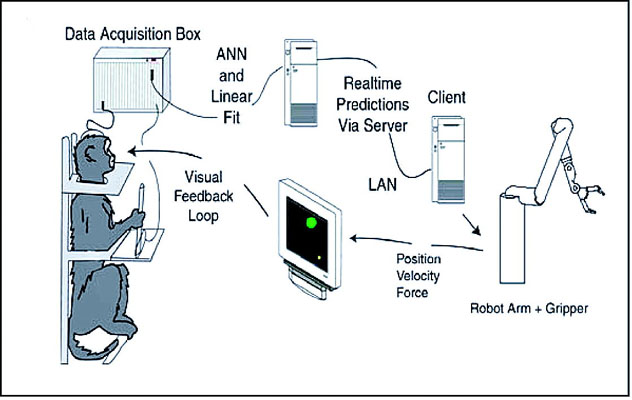
\includegraphics[width=0.8\textwidth] {bilder/apa.jpg}
\caption{A schematic picture of a BCI system used on a monkey~\cite{apa}.}
\label{apa}
\end{figure}

Brain-computer interfaces have mostly been used for controlling prostethic devices for persons that have become blind, have lost limbs or lost control of their motor functions~\cite{lebedev2006brain}, but have in later years also been able to decode pictures from the brain activity~\cite{miyawaki2008visual}.
During the last years BCI equipment has become cheaper and more available to the public market~\cite{legobrain}. The input is however still very sensitive to disturbance, if the user loses focus. To broaden the usage areas of BCI systems more research is needed to ensure stable communications.

The use of BCI comes with a number of ethical questions, the most important of which are side-effects from intrusive BC interfaces, mind reading and mind control. Mind reading could be used for many purposes, some of which are of a questionable ethical nature. Examples of possible applications that might be controversial are neuromarketing to gather data on the neural effects of marketing, or the use of brain readings in interrogation~\cite{10.1371/journal.pbio.1001289, CB:CB252}.

On the one hand mind reading can interfere with the persons privacy, if the mind reading goes on outside the users will. On the other hand, mind reading can be a help or even the only way to communicate for persons that have lost all motor skills and possibly also the use of the eyes.

BCI has the potential to further spread the utilisation of computers in our every-day life, examples of ongoing research are its use in computer gaming~\cite{gurkok2012brain} and thought-controlled cars~\cite{gohring2013semi}. What the future applications could be depends on how well limitations within these techniques can be overcome, it may be that it can replace other interfaces altogether.

